\documentclass[12pt]{article}
\usepackage{graphicx}
\usepackage{amssymb}
\usepackage{epstopdf}
\usepackage{amsmath}
\usepackage{multicol}
\usepackage{tcolorbox}
\usepackage{geometry}
\usepackage{enumitem}
\usepackage{fancyhdr}

\DeclareGraphicsRule{.tif}{png}{.png}{`convert #1 `dirname #1`/`basename #1 .tif`.png}

\textwidth = 6.5 in
\textheight = 9 in
\oddsidemargin = 0.0 in
\evensidemargin = 0.0 in
\topmargin = -23pt
\headheight = 0.0 in
\headsep = 0.0 in
\parskip = 0.2in
\parindent = 0.0in
\pagestyle{fancy}
\pagenumbering{gobble}

\newtheorem{theorem}{Theorem}
\newtheorem{corollary}[theorem]{Corollary}
\newtheorem{definition}{Definition}
%\includegraphics [height=50mm, width=50mm]{PathInt.jpg}
\title{Title} 

\begin{document}
%INSTRUCTOR NOTES

 Name:
 \begin{center}\large{5.3 The Fundamental Theorem and Interpretations}\end{center}

	\begin{tcolorbox}
	\textbf{Total Change Principle}\\
	Let F(t) be some quantity with a continuous rate of change F'(t). Then
	\vspace{10mm}
	\end{tcolorbox}


\begin{enumerate}
\item The graph $v(t)$ is shown.\\
	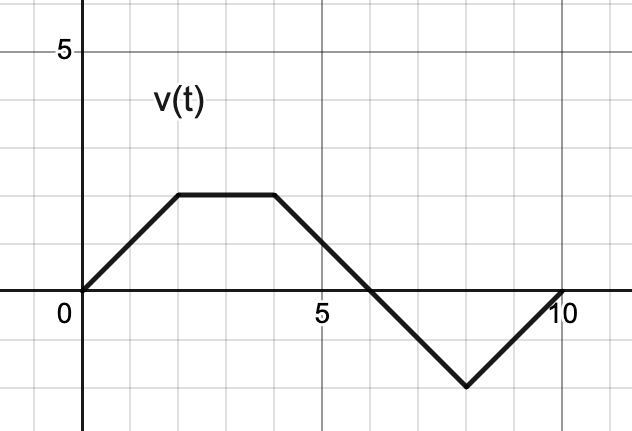
\includegraphics[scale=.3]{5_3_vt}
	\begin{enumerate}
	\item If $v(t)$ is measured in $\frac{km}{hr}$, and $t$ is measured in hours, what are the units of $\int_{0}^{10}v\left(t\right)dt$ and what does it represent?
	\vfill
	\item Find $\int_{0}^{10}v\left(t\right)dt$ and interpret the meaning.
	\vfill
	\item Assuming $v\left(t\right)$measures the velocity of a car starting at position 0 at time 0, sketch a graph of the position of the car as a function of time.
	\vfill
	\item Is there a way to find $\int_{0}^{10}v\left(t\right)dt$ using the position graph?
	\vfill
	\end{enumerate}
\item Pollution is removed from a lake at a rate of $f(t)$ kg/day on day $t$.
	\begin{enumerate}
	\item Explain the meaning of the statement $f(12) = 500$.
\vfill
	\item If $ \displaystyle \int_{5}^{15}f\left(t\right)dt=4000$, give the units of the 5, the 15, and the 4000.
\vfill
	\item Give the meaning of $ \displaystyle \int_{5}^{15}f\left(t\right)dt=4000$.
	\end{enumerate}
	\vfill

\newpage
~
\item Water is leaking out of a tank at a rate of R(t) gallons per hour, where t is measured in hours (see graph to the right).\\

\noindent\begin{minipage}{0.5\textwidth}% adapt widths of minipages to your needs

(a) Write a definite integral that expresses the total amount of water that leaks out in the first two hours.\\

(b) On the graph to the right, shade the region whose area represents the total amount of water that leaks out in the first two hours.\\

(c) Give your best estimate of the amount of water that leaks out of the tank in the first two hours.\\

\end{minipage}%
\hspace{4mm}
\begin{minipage}{0.5\textwidth}
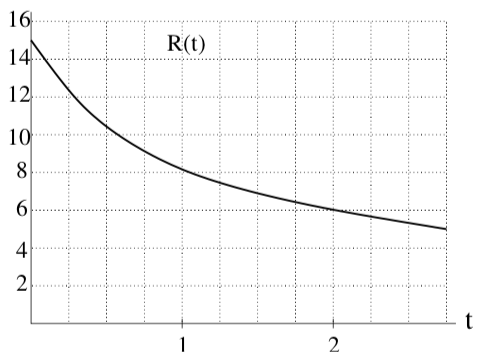
\includegraphics [height=50mm, width=70mm]{5_3_2}
\end{minipage}
\vfill


	\vfill
\item A can of soda is put into a refrigerator to cool. The rate at which the temperature of the soda is changing is
given by $$f(t)= -25e^{-2t} \text{degrees Fahrenheit per hour,}$$
 where $t$ represents the time (in hours) after the soda was placed in the refrigerator.
 	\begin{enumerate}
	\item How fast is the can of soda cooling after 1 hour has passed? Include the appropriate units with your answer.
	\vfill
	\item If the temperature of the can of soda is 60$^\circ$F when it is placed in the refrigerator, estimate the temperature of the can of soda after 3 hours have passed.
	\end{enumerate}
\vfill

\end{enumerate}
\end{document} 

%%%%%%%%%
\item A news broadcast in early 2009 said that the average American’s annual income was changing at a rate of $r(t)$ dollars per month (see the table below), where $t$ is the number of months after January 1, 2009. Estimate the amount that the average American’s income changed in 2009.\\

\begin{tabular}{l | c c c c c c c}
	
	$t$ (months) & 0 &2 & 4 & 6 &8&10&12 \\
	\hline
	$r(t)$ (dollars per month) & 40.00 & 40.16 & 40.32& 40.48 & 40.64 & 40.81 & 40.97\\
	
	\end{tabular}

\begin{enumerate}
\item Let $s(t)$ be the position, in feet, of a car along a straight east/west highway at time $t$ seconds. Positive values of s indicate eastward displacement of the car from home, and negative values indicate westward displacement. Let $v(t)$ represent the velocity of this same car, in feet per second, at time $t$ seconds (see graph).\\
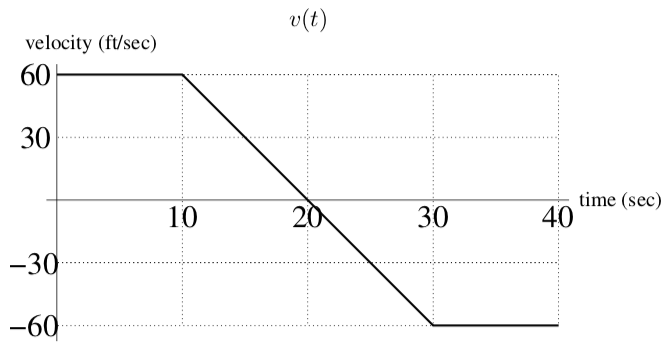
\includegraphics [height=50mm, width=80mm]{5_3_velocity}
	\begin{enumerate}
	\item Use the velocity graph above to help you fill in the chart below.\\
	\begin{tabular}{c|c@{\hskip 8mm}c@{\hskip 8mm}c@{\hskip 8mm}c@{\hskip 8mm}c@{\hskip 8mm}}
	
	$t$ & 0 &10  & 20 & 30 &40 \\
	
	\hline
	&&&&&\\
	$s(t)$ &  & & & &  \\
	&&&&&\\
	\end{tabular}
\vfill
	\item Fill in the chart below.\\
		\begin{tabular}{l@{\hskip 1.5in}|l@{\hskip 0.5in}c}
	Integral of Velocity & Change in Position\\
	\hline
	$\displaystyle \int_0^{10} v(t)\,dt =$ &$s(10)-s(0)$\\
	&\\
	$\displaystyle \int_0^{20} v(t)\,dt =$ &$s(20)-s(0)$\\
	&\\
	$\displaystyle \int_{20}^{40} v(t)\,dt =$ &$s(40)-s(20)$\\
	&\\
	$\displaystyle \int_0^{40} v(t)\,dt =$ &$s(40)-s(0)$\\
	&\\
	\end{tabular}
	\vfill
	\end{enumerate}
\begin{tcolorbox}
\textbf{Warm-up: } Solve the following equations for $t$.
\begin{multicols}{2}
\begin{enumerate}
\item $(t+1)^2=9$
\item $tx+x^2=5$
\end{enumerate}
\end{multicols}
\end{tcolorbox}

MINIPAGE
\noindent\begin{minipage}{0.3\textwidth}% adapt widths of minipages to your needs
try 1
\end{minipage}%
\hspace{40mm}
\begin{minipage}{0.6\textwidth}
a) $f'(2)=$\\\

b) $f'(4)=$\\

c) $f'(6)=$\\

d) $f'(7)=$\\

e) $f'(8)=$
\end{minipage}
